\documentclass[12pt]{extarticle}
\usepackage{tempora}
\usepackage[T1, T2A]{fontenc}
\usepackage[utf8]{inputenc}
\usepackage[english, ukrainian]{babel}
\usepackage{geometry}
\usepackage{graphicx}
\usepackage{multirow}
\usepackage{multicol}
\usepackage{float}
\graphicspath{{/home/artem/Pictures}}
\geometry
{
    a4paper,
    left=30mm,
    top=15mm,
    right=20mm,
    bottom=15mm,
}

\begin{document}
\begin{titlepage}
    \begin{center}
        \textbf{\normalsize{\MakeUppercase{
            Міністерство Освіти і науки України
            Національний університет "Львівська політехніка"
        }}}

        \begin{flushright}
        \textbf{ІКНІ}\\
        Кафедра \textbf{ПЗ}
        \end{flushright}
        \vspace{15mm}

        \includegraphics[width=0.4\textwidth]{lpnu_logo.png}

        \vspace*{\fill}

        \textbf{\normalsize{\MakeUppercase{Звіт}}}
            
        До лабораторної роботи №2

        \textbf{на тему:} “ Метод сортування Шелла.”

        \textbf{з дисципліни:} "Алгоритми і структури даних”
            
        \vspace*{\fill}

        \begin{flushright}

            \textbf{Лектор:}\\
            доцент кафедри ПЗ\\
            Коротєєва Т. О.\\
            \vspace{12pt}

            \textbf{Виконав:}\\
            студент групи ПЗ-24\\
            Губик А. С.\\
            \vspace{12pt}

            \textbf{Прийняв:}\\
            асистент кафедри ПЗ\\
            Вишнеський О. К.\\
        \vspace{12pt}
        \end{flushright}

        Львів -- 2023
            
            
    \end{center}
\end{titlepage}

\subsection*{Тема роботи} 
Метод сортування Шелла.

\subsection*{Мета роботи} Вивчити алгоритм сортування Шелла. 
Здійснити програмну реалізацію алгоритму сортування Шелла. 
Дослідити швидкодію алгоритму сортування Шелла.

\subsection*{Індивідуальне завдання}
Задано матрицю дійсних чисел. Впорядкувати (переставити) її стовпці за зростанням значень їх перших елементів.

\subsection*{Теоретичні відомості}
Сортування Шелла (англійською «Shell Sort») — це алгоритм сортування, що є узагальненням сортування включенням.

Алгоритм базується на двох тезах:

Сортування включенням ефективне для майже впорядкованих масивів.
Сортування включенням неефективне, тому що переміщує елемент тільки на одну позицію за раз.
Тому сортування Шелла виконує декілька впорядкувань включенням, кожен раз порівнюючи і переставляючи елементи, що знаходяться на різній відстані один від одного.

Сортування Шелла не є стабільним.

Сортування Шелла названо начесть автора — Дональда Шелла, який опублікував цей алгоритм у 1959 році. 

На початку обираються m елементів: d1, d2, …, dm, причому d1 > d2 > … > dm = 1.

Потім виконується m впорядкувань методом включення, спочатку для елементів, що стоять через d1, потім для елементів через d2і так далі до dm = 1.

Значення   d1  = m/2.

Ефективність досягається тим, що кожне наступне впорядкування вимагає меншої кількості перестановок, оскільки деякі елементи вже стали на свої місця.

Оскільки dm = 1, то на останньому кроці виконується звичайне впорядкування включенням всього масиву, а отже кінцевий масив гарантовано буде впорядкованим.

Час роботи залежить від вибору значень елементів масиву d. Існує декілька підходів вибору цих значень:
\subsection*{Покроковий опис}

\begin{enumerate}

\item \textbf{Принцип сортування:} Далі над масивом матиметься на увазі перший
ряд таблиці, сортувати ми будемо лише його, впорядккуванням стовпців займатиметься інша функція. 

\item \textbf{Вибір послідовності проміжків:} Перший крок в Shell Sort -- це 
вибір послідовності проміжків (інтервалів). Вибір послідовності 
проміжків - це важлива частина алгоритму, яка може значно вплинути 
на його ефективність. Загальні послідовності проміжків включають 
послідовність Кнута (1, 4, 13, 40, ...), послідовність Седжвіка та 
інші. Вибрані проміжки використовуються для розбиття масиву на менші
 підмасиви.
\item \textbf{Початок із найбільшим проміжком:}  Починаючи з найбільшого проміжку,
 алгоритм розбиває масив на підмасиви. Наприклад, якщо перший проміжок
  - 4, то він розділить масив на підмасиви довжиною 4, де елементи на
   позиціях 0, 4, 8 і т.д. утворюють один підмасив, а елементи на позиціях
    1, 5, 9 і т.д. утворюють інший.
\item \textbf{Сортування підмасивів:} Для кожного підмасиву виконується сортування 
вставками. Це означає порівняння та обмін елементів, які розташовані 
на "проміжку" позиціях один від одного всередині кожного підмасиву.
 Мета - частково відсортувати кожен підмасив.

\item \textbf{Зменшення проміжка:} Після сортування 
підмасивів алгоритм зменшує розмір проміжка і повторює процес. Мета --
 послідовно зменшувати розмір проміжка, поки він не стане рівним 1.
\item \textbf{Завершальний прохід:}Завершальний прохід алгоритму -- це звичайне 
сортування вставками із проміжком 1. Цей крок допомагає докладно 
відсортувати масив і перетворити його на відсортований масив.

\item \textbf{Завершення:}  Після завершального проходу з проміжком 1 
весь масив відсортований. Алгоритм Shell Sort завершується.
\end{enumerate}

\subsection*{Вихідний код}

{\fontfamily{pcr}\selectfont

\begin{verbatim}
    
    #include <iostream>
    #include <vector>
    #include <cstdlib>
    #include <ctime>
    #include <algorithm>
    #include <chrono>
    
    // Function to perform Shell sort on an array of pairs
    void shellSort(std::vector<std::pair<float, int>>& arr) {
        int n = arr.size();
    
        for (int gap = n / 2; gap > 0; gap /= 2) {
            for (int i = gap; i < n; i++) {
                std::pair<float, int> temp = arr[i];
                int j;
    
                for (j = i; j >= gap && arr[j - gap].first > temp.first; j -= gap) {
                    arr[j] = arr[j - gap];
                }
    
                arr[j] = temp;
            }
            std::cout << "Step: ";
            for (size_t i = 0; i < n; i++)
            {
                std::cout << arr[i].first << ' ';
            }
            std::cout << '\n';
            
        }
    
    }
    
    // Function to print the matrix
    void printMatrix(const std::vector<std::vector<float>>& matrix) {
        int n = matrix.size();
        int m = matrix[0].size();
    
        for (int i = 0; i < n; i++) {
            for (int j = 0; j < m; j++) {
                std::cout << matrix[i][j] << "\t";
            }
            std::cout << std::endl;
        }
    }
    
    int main() {
        int n, m;
    
        // Get user input for the matrix dimensions
        std::cout << "Enter the number of rows (n): ";
        std::cin >> n;
        std::cout << "Enter the number of columns (m): ";
        std::cin >> m;
    
        // Create a 2D matrix
        std::vector<std::vector<float>> matrix(n, std::vector<float>(m));
    
        // Fill the matrix with random float numbers
        std::srand(static_cast<unsigned int>(std::time(nullptr)));
        for (int i = 0; i < n; i++) {
            for (int j = 0; j < m; j++) {
                matrix[i][j] = static_cast<float>(std::rand()) / static_cast<float>(RAND_MAX) * 100.0f;
            }
        }
    
        // Display the original matrix
        std::cout << "Original Matrix:" << std::endl;
        printMatrix(matrix);
    
        // Create a vector of pairs to store the values in the first row along with their original column indices
        std::vector<std::pair<float, int>> firstRowWithIndex;
        for (int j = 0; j < m; j++) {
            firstRowWithIndex.push_back({matrix[0][j], j});
        }
    
        // Measure the sorting time
        auto startTime = std::chrono::high_resolution_clock::now();
    
        // Sort the vector of pairs based on the values in the first row using Shell sort
        shellSort(firstRowWithIndex);
    
        auto endTime = std::chrono::high_resolution_clock::now();
        std::chrono::duration<double> duration = endTime - startTime;
    
        // Rearrange the columns of the matrix based on the sorted indices
        std::vector<std::vector<float>> sortedMatrix(n, std::vector<float>(m));
        for (int i = 0; i < n; i++) {
            for (int j = 0; j < m; j++) {
                sortedMatrix[i][j] = matrix[i][firstRowWithIndex[j].second];
            }
        }
    
        // Display the matrix sorted by the values in the first row
        std::cout << "Matrix Sorted by First Row:" << std::endl;
        printMatrix(sortedMatrix);
    
        std::cout << "Sorting Time: " << duration.count() << " seconds" << std::endl;
    
        return 0;
    }
    
\end{verbatim}
}
\vspace{12pt}
\begin{figure}[H]
    \centering
    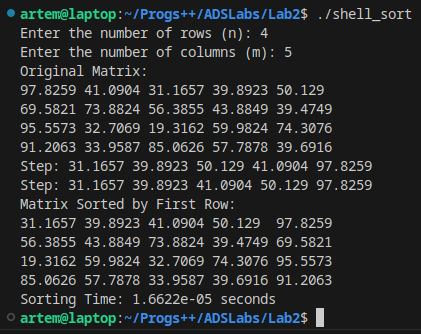
\includegraphics[width=0.90\textwidth]{Screenshot_20231010_195127.png}
    \caption{}
\end{figure}
\subsection*{Висновок} 
Ідея застосування проміжків в Shell 
Sort полягає в тому, що він використовує ефективність сортування
 вставками для майже відсортованих підмасивів. Початкове сортування
  підмасивів з відносно великим проміжком швидко зменшує кількість
   безладу в масиві, що робить завершальне сортування значно швидшим.
\end{document}
